%%%%%%%%%%%%%%%%%%%%%%%%%%%%%%%%%%%%%%%%%
% Thin Sectioned Essay
% LaTeX Template
% Version 1.0 (3/8/13)
%
% This template has been downloaded from:
% http://www.LaTeXTemplates.com
%
% Original Author:
% Nicolas Diaz (nsdiaz@uc.cl) with extensive modifications by:
% Vel (vel@latextemplates.com)
%
% License:
% CC BY-NC-SA 3.0 (http://creativecommons.org/licenses/by-nc-sa/3.0/)
%
%%%%%%%%%%%%%%%%%%%%%%%%%%%%%%%%%%%%%%%%%

%----------------------------------------------------------------------------------------
%	PACKAGES AND OTHER DOCUMENT CONFIGURATIONS
%----------------------------------------------------------------------------------------

\documentclass[11pt]{article} % Font size (can be 10pt, 11pt or 12pt) and paper size (remove a4paper for US letter paper)

\usepackage[utf8]{inputenc} % Set utf8 code
\usepackage[protrusion=true,expansion=true]{microtype} % Better typography
\usepackage[portuguese]{babel}
\usepackage{graphicx} % Required for including pictures
\usepackage{wrapfig} % Allows in-line images
\usepackage{hyperref}

\usepackage{mathpazo} % Use the Palatino font
\usepackage[T1]{fontenc} % Required for accented characters
\usepackage{wallpaper}
\usepackage[font={color=white,bf},figurename=Fig.,labelfont={it}]{caption}
\usepackage{lipsum, xcolor, etoolbox}
\hypersetup{
    colorlinks=false,
    pdfborder={0 0 0},
}

\linespread{1.05} % Change line spacing here, Palatino benefits from a slight increase by default

\makeatletter
\renewcommand\@biblabel[1]{\textbf{#1.}} % Change the square brackets for each bibliography item from '[1]' to '1.'
\renewcommand{\@listI}{\itemsep=0pt} % Reduce the space between items in the itemize and enumerate environments and the bibliography

\renewcommand{\maketitle}{ % Customize the title - do not edit title and author name here, see the TITLE block below
\begin{center} % Right align
{\LARGE\@title} % Increase the font size of the title

\vspace{20pt} % Some vertical space between the title and author name

\end{center}
}
\patchcmd{\ps@plain}{\thepage}{\textcolor{white}{\thepage}}{}{}

\makeatother
\begin{document}
\ThisTileWallPaper{\paperwidth}{\paperheight}{res/wallpaper_header.jpg}
\color{white}
\pagestyle{plain}

\begin{titlepage}
 \vfill
  \begin{center}
   {\textbf{{{\Huge  Strife Of Mythology Tower Defense}}}} \\
   \\[6cm]


   {{\huge Documento de visão}}\\[6cm]

   \hspace{.45\textwidth} %posiciona a minipage
  \vfill

\vspace{2cm}

\large \textbf{Brasília}

\large \textbf{Abril de 2016}
\end{center}
\end{titlepage}
\newpage
%----------------------------------------------------------------------------------------
%	DOC BODY
%----------------------------------------------------------------------------------------

\TileWallPaper{\paperwidth}{\paperheight}{res/wallpaper_body.jpg}
\color{white}
\section*{Apresentação}

\paragraph{}\textbf{Strife of Mythology é um \textit{Tower Defense} de tema mitológico. Neste jogo as suas torres evoluirão a medida que o jogador acumula pontos no decorrer da partida, tornando-as cada vez mais avançadas e poderosas. Tais torres poderão ser de diferentes tipos, cada uma com a sua peculiaridade, as quais dependem do personagem escolhido, sendo que cada personagem possui as suas próprias torres}

\section*{Resumo}

\paragraph{}\textbf{Conheça um mundo mágico dominado por criaturas mitológicas poderosas, neste mundo inimigos que desejam avançar sobre o território da humanidade, destruindo tudo o que encontrar pelo caminho.}

\paragraph{}\textbf{Porém do lado da humanidade os Deuses mesmo imortais ouviram as preces dos humanos e partiram para guerra, com o objetivo de impedir o avanço destes monstros, através de torres mágicas com diversos ataques na tentativa de destruit estes monstros.}

\usepackage[opções]{subfigure}

\begin{figure}[!htp]
\centering
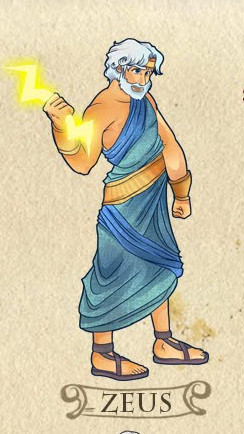
\includegraphics[scale=0.3]{res/zeus.png} \quad
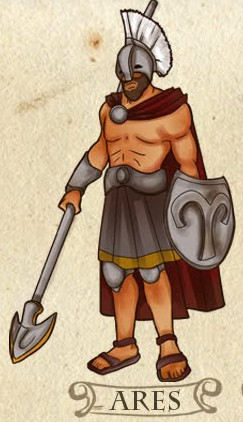
\includegraphics[scale=0.3]{res/ares.png} \quad
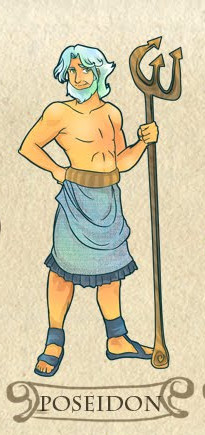
\includegraphics[scale=0.3]{res/poseidom.png} \quad
\label{Nave Espacial}
\center
\caption{Deuses Zeus, Ares e Poseidom}

\end{figure}

\paragraph{}\textbf{No lado da humanidade três Deuses deceram ao mumdo dos mortais para destrui as levas de montros que apareceram na guerra, sendo eles \textit{\textbf{Zeus}, \textbf{Ares} e \textbf{Poseidon}}.}

\section*{Principais características}
\subsection{Modo Endurece}\paragraph{O jogo nunca acaba a não ser que o jogador seja derrotado, quando determinada quantidade de inimigos conseguirem atravesar o campo, porém o jogo terá três mapas, as quais são abertas a medidada que o jogador alcança uma grande quantidades de pontos na fase.} 

\subsection{Torres}
\paragraph{Cada deus tem as suas torres, cada uma contendo uma especialidade diferente, porém estas torres também possuem a sua desvantagem.
\begin{itemize}
\item Zeus tem torres com dano alto(raios) mas com ataque speed pequeno, o que torna ele bom contra unidades tanks e fraco contra unidades em massas.
\item Hades tem torres que são boas contra unidades aéreas.
\item Poseidon tem torres que atacam em áreas(ondas) e causam dano no inimigos no espaço próxima a torre.
\end{itemize}
}
\paragraph{As torres possuem um sistema de \textit{Tiers}, esta hierarquia é distribuída em três níveis, possuindo uma barra de desempenho, que ao decorrer do jogo a mesma com o progresso do jogador será preenchida, liberando acesso a torre de nível superior} 
\paragraph{Caso se arrependa da compra da torre é possível revende-la, por um preço inferior ao pago em determinados períodos no jogo.}

\subsection{Um Player}
\paragraph{SoMTD terá somente um jogador.}

\subsection{Sem Mazing}
\paragraph{Os monstros fazem sempre o mesmo caminho, que não poderá ser bloqueado.}

\subsection{Respawn Fixo}
\paragraph{Os monstros sempre nascem no mesmo lugar.}

\subsection{Vida}
\paragraph{O jogador começa com um valor fixo de pontos de vida, este será um barra de \textit{HP(Health Point} assim quando os inimigos conseguirem atravessar o caminho esta barra decairá, não sendo possível reverter esse valor.}

\begin{figure}[!htp]
\centering
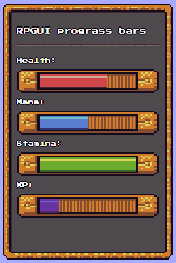
\includegraphics[scale=0.3]{res/hp.png}
\caption{Exemplo de Hp}
\label{Mecânicas}
\end{figure}


\section*{Esquema de Controle e Interface}
\paragraph{Strife of Mythology deve ser jogado com o aux´ilio de um mouse e teclado. Os atalhos para acesso rápido( também chamados de hotkeys) facilitarão  a jogabilidade, e serão possíveis com a utilização de um teclado (esses atalhos irão por exemplo, possibilitar qual torre construir, revender, entre outras coisas)}.

\paragraph{Com o mouse, o jogador escolhe essecialmente as torres e as posições de construção.}
Botão esquerdo:
\begin{figure}[!htp]
\begin{center}
  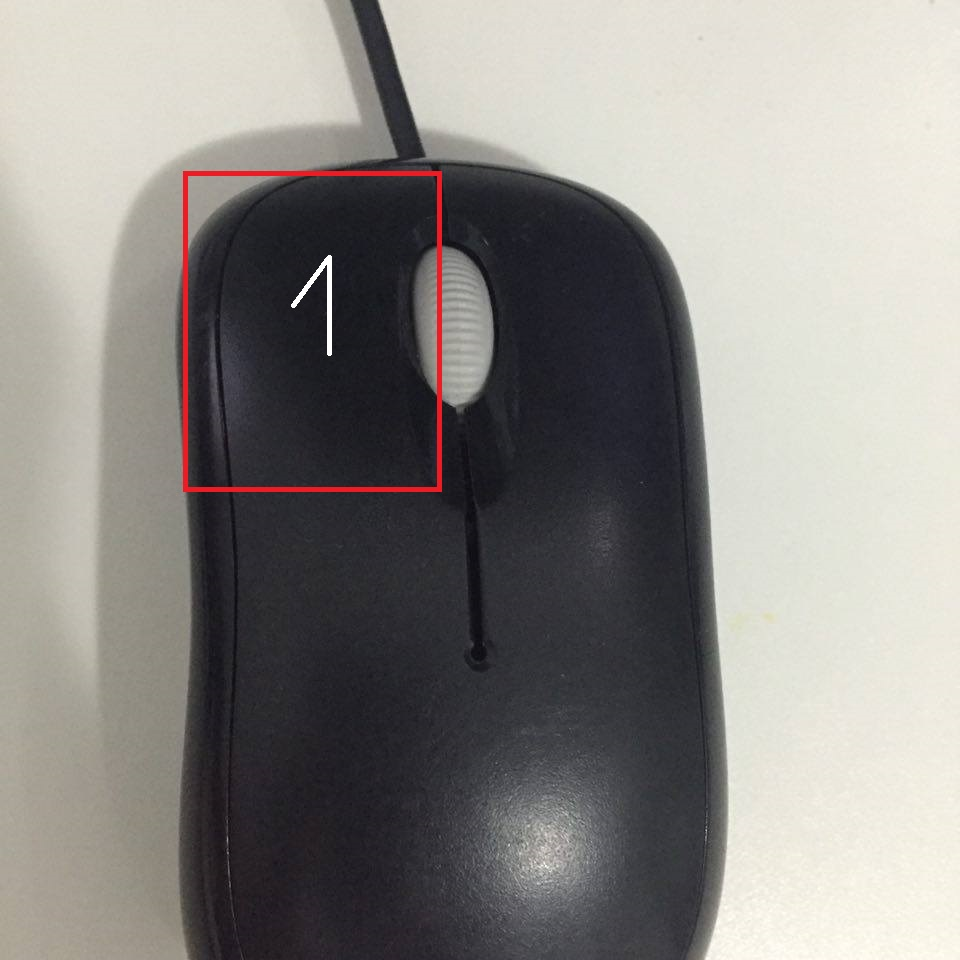
\includegraphics[scale=0.1]{res/mouse.png} \quad
\caption{Periféricos de entrada} \label{gdimotes}
\end{center}
\end{figure}
\begin{enumerate}
\item Botão esquerdo:
\begin{itemize}
\item Seleção do menu;
\item Escolha de Deuses;
\item Seleção de torres;
\end{itemize}
\end{enumerate}

\section*{Público Alvo}
\begin{figure}[!htp]
\begin{center}
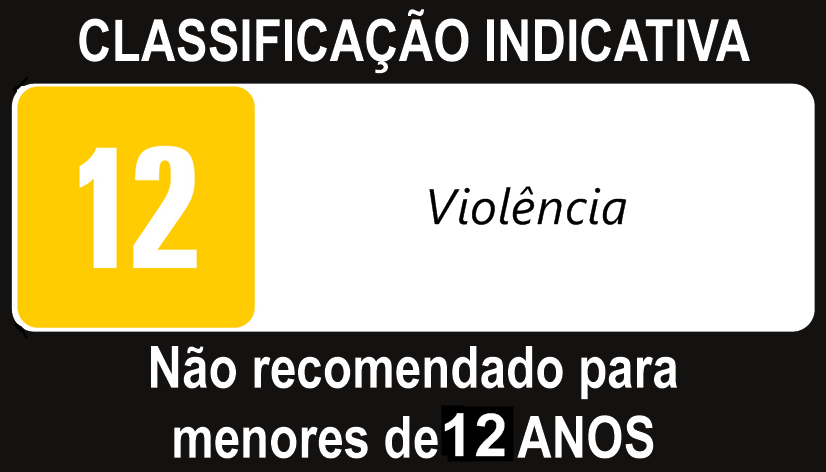
\includegraphics[scale=0.1]{res/12anos.png} 
\caption{classificação indicativa} \label{gdimotes}
\end{center}
\end{figure}
\paragraph{O público alvo, são pessoas de qualquer faixa etária, que gostam de experimentar jogos novos, mais especificamente no subgênero Tower Defense. Porém como o jogo pode apresentar cenas violentas a classificação ficou em 12 anos.}

\section*{Plataformas Alvo}
\paragraph{Tem-se como plataformas alvo, o windows e o Linux.}
\begin{figure}[!htp]
\begin{center}
  
\includegraphics[scale=0.1]{res/windows.png} \quad
  
\includegraphics[scale=0.3]{res/linux.png} \quad
\caption{Plataformas} \label{gdimotes}
\end{center}
\end{figure}
 
\section*{Recursos tecnológicos notáveis}

\begin{figure}[!htp]
\begin{center}
  
\includegraphics[scale=0.04]{res/audacity.png} \quad
  
\includegraphics[scale=0.3]{res/adobe_illustrator.png} \quad
  
\includegraphics[scale=0.25]{res/Sdl-logo.png} \quad
  
\includegraphics[scale=0.3]{res/Sublime_Text_Logo.png} \quad
  
\includegraphics[scale=0.2]{res/cpp.png} \quad
  
\includegraphics[scale=0.13]{res/git.png} \quad
  
\includegraphics[scale=0.5]{res/linux.png} \quad
\caption{Recursos Tecnológicos} \label{gdimotes}
\end{center}
\end{figure}

\section*{Informações de contato}
{\Huge \textbf{strifeofmythology@gmail.com}}

\end{document}
